\chapter{Method}
\label{chapter:method}
At its core, our method formulates the necessary and sufficient conditions for quadrangulating a triangle-mesh by parametrization (integer-grid maps \cite{bommes:hal-00862648}), as a smooth unconstrained optimization problem using periodic functions. Our main objective function is a weighted sum of smooth penalty functions (also can be regarded as sub-objective functions), of which their weights are controllable by the user. We believe that this approach is more suitable for 3D design and modeling tools since the quadrangulation process is continuous with the user constantly in the loop. This approach is also easily extensible by introducing additional smooth terms (sub-objectives) into the main objective, which can represent custom requirements of which the parameterization has to fulfill. Moreover, since the weights are controllable, the quadrangulation process can be executed in any desired order (e.g. achieve a seamless parametrization before handling singular points). That's why we decided to call our approach \emph{Smooth and Interactive Parametrization-Based Quadrangulation}: \emph{Smooth} because we're using a smooth objective, \emph{Interactive} because small changes are immediately reflected to the user, and \emph{Parametrization-Based} because we solve a global parametrization problem. This chapter is organized as following: In section \ref{integer-grid-maps} we describe in detail the notion of integer-grid maps, and the necessary and sufficient conditions under which such maps form a quad mesh on the 3D surface. In section \ref{section:quad_distortion_cond} we briefly describe how to we cope with quad-distortion in order to maximize mesh quality. In section \ref{section:smooth_objective_functions} we describe the formulation of the integer-grid maps conditions as smooth penalty functions. In section \ref{section:optimization} we derive the gradient and Hessian of our main objective function. In section \ref{section:initialization} we briefly describe how we initialize the optimization process by cutting the input mesh open into a triangle-soup on the parametrization domain, and in section \ref{section:graphic_user_interface} we briefly describe the implementation details and the main components of the graphic user interface we provide for the user.
\section{Integer Grid Maps}
\label{integer-grid-maps}
The necessary and sufficient conditions for a parametrization mapping to form a valid quad mesh on the mesh's 3D surface are:
\begin{enumerate}
\item Seamless Condition
\item Singular Points Condition
\item Consistent Orientation Condition
\end{enumerate}
\subsection{Seamless Condition}
\label{section:seamless_cond}
The transition function $g_{ij}$ between two half-edges $e_i$ and $e_j$ on the parameterization domain that corresponds to the same surface edge that is part of a cut seam, has to be an integer-grid automorphism given by:
\begin{equation}\label{transition_g_ij}
\begin{split}
e_j = R^{r_{ij}}_{90^\circ}e_i + \vec{t}_{ij}
\end{split}
\end{equation}
Where  $r_{ij} \in \{0,1,2,3\}$ and $\vec{t}_{ij} \in \mathbb{Z}^2$. Figures \ref{fig:translation_req}, \ref{fig:angle_req} and \ref{fig:length_req} visually demonstrate the 3 requirements encoded by the seamless condition.
\begin{figure}[ht]
\centering
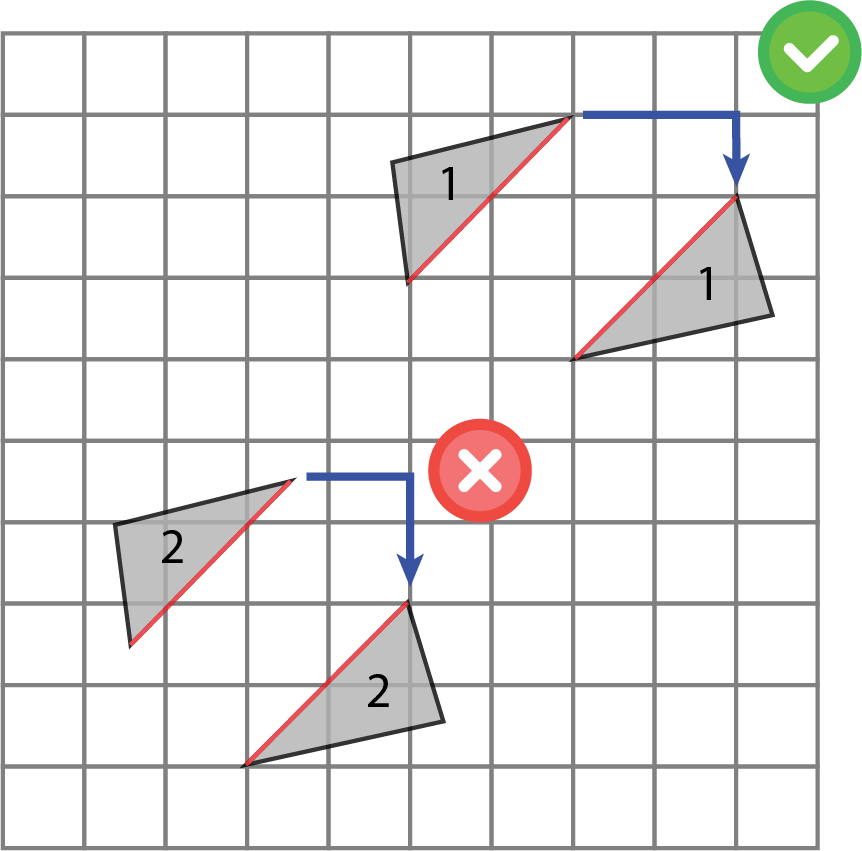
\includegraphics[width=6cm]{figures/seamless/translation.png}
\caption[The Translation Requirement]{The transition function $g_{ij}$, described by equation \ref{transition_g_ij}, should impose an integer translation between the two half edges.}
\label{fig:translation_req}
\end{figure}
\begin{figure}[ht]
\centering
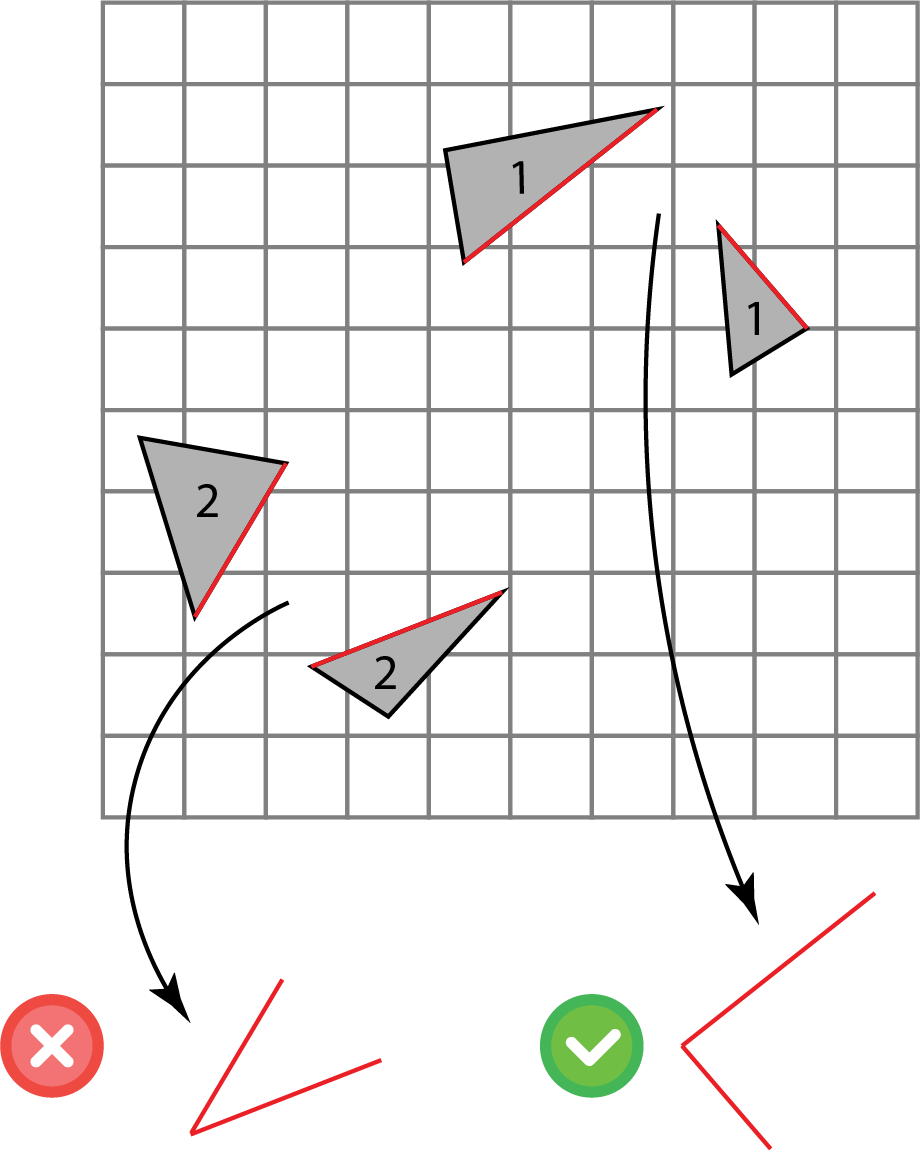
\includegraphics[width=6cm]{figures/seamless/angle.png}
\caption[The Angle Requirement]{The transition function $g_{ij}$, described by equation \ref{transition_g_ij}, should impose a $\frac{\pi}{2}k$ rotation between the two half edges.}
\label{fig:angle_req}
\end{figure}
\begin{figure}[ht]
\centering
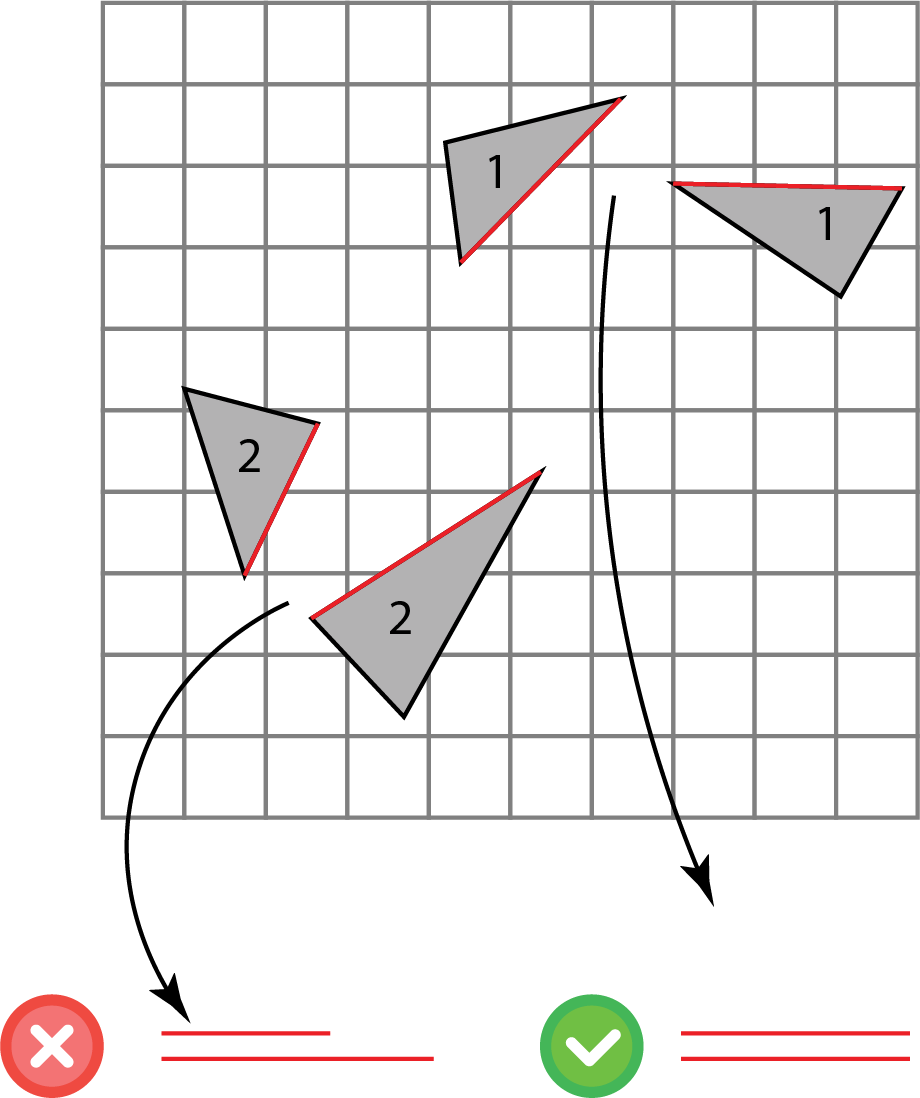
\includegraphics[width=6cm]{figures/seamless/length.png}
\caption[The Length Requirement]{The transition function $g_{ij}$, described by equation \ref{transition_g_ij}, should implicitly match the length of the two half edges.}
\label{fig:length_req}
\end{figure}
\subsection{Singular Points Condition}
\label{section:singular_points_cond}
Before we define what the singular-points condition is, we first have to define how a singular vertex is characterized on the parametrization domain. A singular-vertex (valence $\neq 4$) on the mesh's surface, will be characterized on the parametrization domain by a non-zero angular defect. The angular defect is measured by $2\pi - \sum_{i=1}^k \theta_i$ and $\pi - \sum_{i=1}^k \theta_i$ for interior and boundary surface vertices, respectively, where $k$ is the number of twin-vertices on the the parametrization domain that correspond to the singular-vertex on the mesh's surface, and $\theta_i$ is the angle adjacent to twin-vertex $v_i$.
Having the right definitions, the singular-points condition require that all twin-vertices of singular points will be located on integer locations. Formally, given the set $V$ of all twin-vertices on the domain the that correspond to the a singular vertex on the mesh's surface, we require that:
\begin{equation}\label{eq:singular_points_cond}
\begin{split}
\forall u \in V: u \in \mathbb{Z}^2
\end{split}
\end{equation}
Figure \ref{fig:singular_points_req} demonstrate this condition visually.
\begin{figure}[ht]
\centering
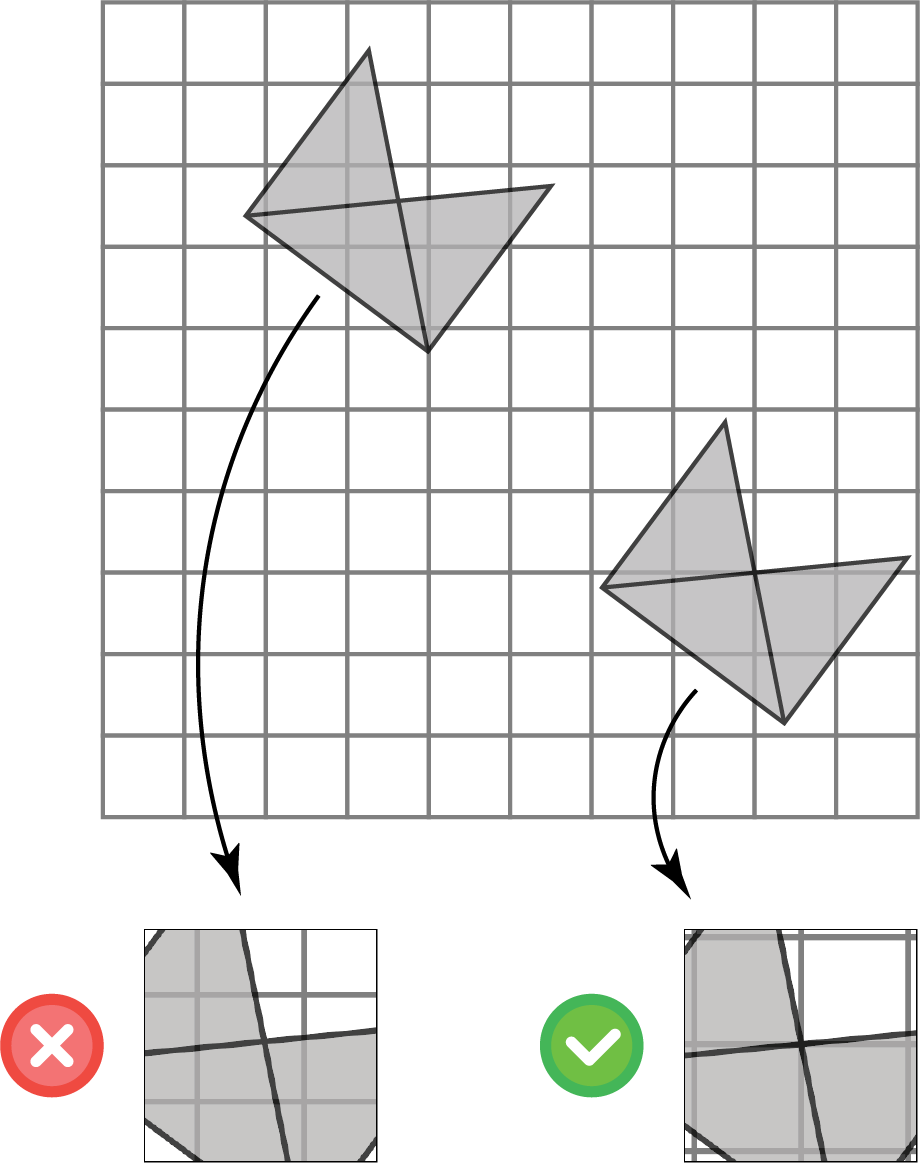
\includegraphics[width=6cm]{figures/singular_points/singularity.png}
\caption[The Singular Points Requirement]{Domain vertices that correspond to the same singular point should be positioned at a integer locations (grid points). In this illustration, the angular defect is $\frac{\pi}{2}$.}
\label{fig:singular_points_req}
\end{figure}
\subsection{Consistent Orientation Condition}
\label{section:consistent_otrientation_cond}
All triangles on the parameterization domain should have the same orientation. In other words, the transition function should not allow triangle flips. Figure \ref{fig:orientation_req} demonstrate this condition visually.
\begin{figure}[ht]
\centering
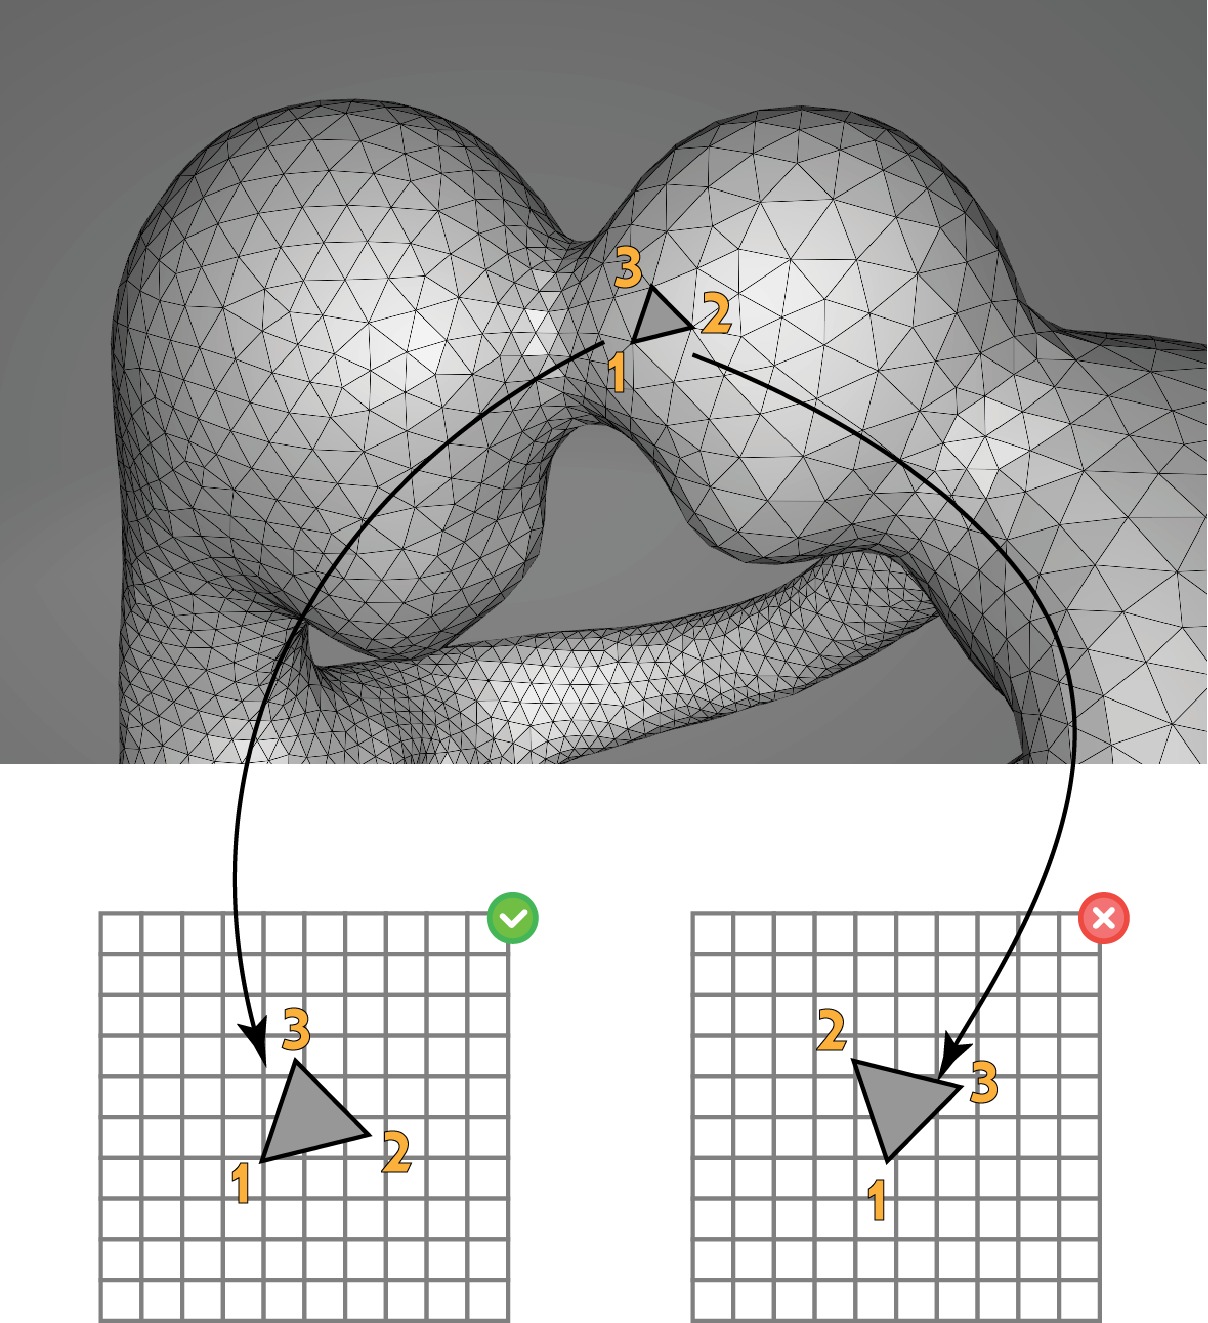
\includegraphics[width=6cm]{figures/orientation/orientation.png}
\caption[The Orientation Requirement]{The left triangle follows the same counter clockwise orientation as its image on the mesh's surface. On the other hand, the vertices of the triangle on the right follows a clockwise orientation.}
\label{fig:orientation_req}
\end{figure}
\section{Quad Distortion}
\label{section:quad_distortion_cond}
The fulfilment of the integer-grid maps conditions do guarantee that the isolines of the 2D Cartesian grid form a valid quad-mesh on the 3D mesh's surface, however, we do have to consider at what cost. There are many possible integer-grid maps that transform a given triangle-mesh into a quad-mesh. Amongst them, we would like to pick the one that satisfies our desired set of additional requirements. In order to meet this desiderata, we have to pay with shape distortion of the triangles that make up the parametrization domain. Ultimately, we would like to find a map that fits our needs and minimizes the triangles distortion, since a distorted triangle renders a distorted isoline on the input mesh surface, which eventually affects the quality of the extracted quads that correspond to that triangle. Therefore, in addition to the integer-grid maps conditions, we add an additional implicit core requirement, which demands to find a mapping that minimizes triangle distortion. Figure \ref{fig:distortion_req} demonstrate this requirement visually.
\begin{figure}[ht]
\centering
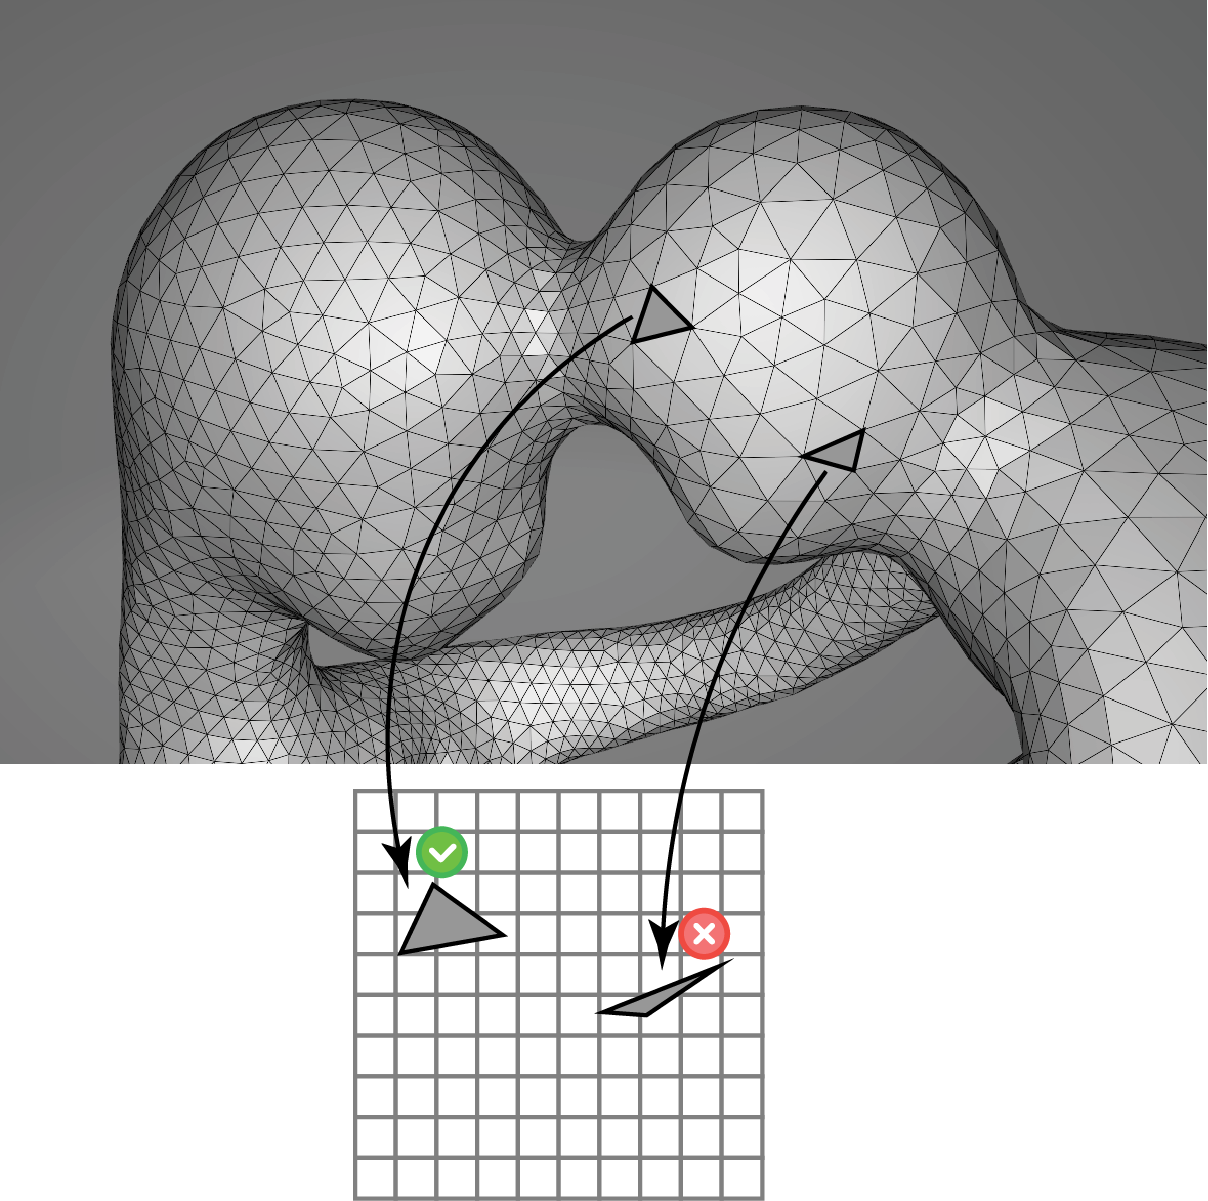
\includegraphics[width=6cm]{figures/distortion/distortion.png}
\caption[The Orientation Requirement]{The left triangle has a little shape distortion compared with its original version on the input-mesh's surface, in contrast with the right triangle, which clearly express a high shape distortion compared with its original version}
\label{fig:distortion_req}
\end{figure}
\section{Smooth Penalty Functions}
\label{section:smooth_objective_functions}
In this section, we present our smooth penalty function formulations for conditions \ref{section:seamless_cond}, \ref{section:singular_points_cond}, \ref{section:consistent_otrientation_cond} and requirement \ref{section:quad_distortion_cond}, as presented in the previous sections. Please note, in the following sections and subsections below, we denote by $\mathrm{x}\left(v\right)$, $\mathrm{y}\left(v\right)$ the $x$ and $y$ coordinates of a given domain vertex $v$.
\subsection{The Seamless Condition's Penalty Functions}
The seamless condition can be expressed by three smooth penalty functions $P_{angle}$, $P_{length}$ and $P_{translation}$, that penalize violations in angle, length and translation, respectively, for a given pair of half-edges. In the following three paragraphs, we define those tree penalty functions, and assume we're given two half-edges, in the parametrization domain, denoted by $e_i = \left(v_i^1,v_i^2\right)$ and $e_j = \left(v_j^1,v_j^2\right)$, where for for $k \in \left\{i,j\right\}$, $v_k^1$ and $v_k^2$ are the two domain vertices that constitutes half-edge $k$, and for $k \in \left\{1,2\right\}$, $v_i^k$ and $v_j^k$ are twin-vertices.
\paragraph{Angle Penalty}
\label{paragraph:angle_penalty_function_method}
We define $P_{angle}$ as follows:
\begin{equation}\label{eq:angle_penalty}
\begin{split}
P_{\mathrm{angle}}\left(e_i,e_j\right) = \mathrm{sin} \bigg( 4\Big(\theta\left(e_i\right) - \theta\left(e_j\right)\Big) - \frac{\pi}{2}\bigg) + 1
\end{split}
\end{equation}
Where $\theta\left(e_k\right) = \mathrm{atan2}\Big(\mathrm{y}\left(v_k^2\right) - \mathrm{y}\left(v_k^1\right), \mathrm{x}\left(v_k^2\right) - \mathrm{x}\left(v_k^1\right)\Big)$ is the angle formed by half-edge $e_k = \left(v^1_k, v^2_k\right)$ with the positive \emph{x-axis} direction, when treated as a vector based at $v_k^1$ and heading $v_k^2$, for $k \in \left\{i,j\right\}$. Therefore, the expression $\theta\left(e^i\right) - \theta\left(e^j\right)$ yields the signed angle between the two half-edges. Figure \ref{fig:angle_penalty} shows a plot of the angle penalty function for a range of $\theta$ values. It is easy to see that the angle penalty is minimized when the angle discrepancy between the two half-edges is an integer multiple of $\frac{\pi}{2}$, as required by the seamless condition. Please note, equation \ref{eq:angle_penalty} yields only non-negative values due to the introduction of the $+1$ term.
\begin{figure}[ht]
\centering
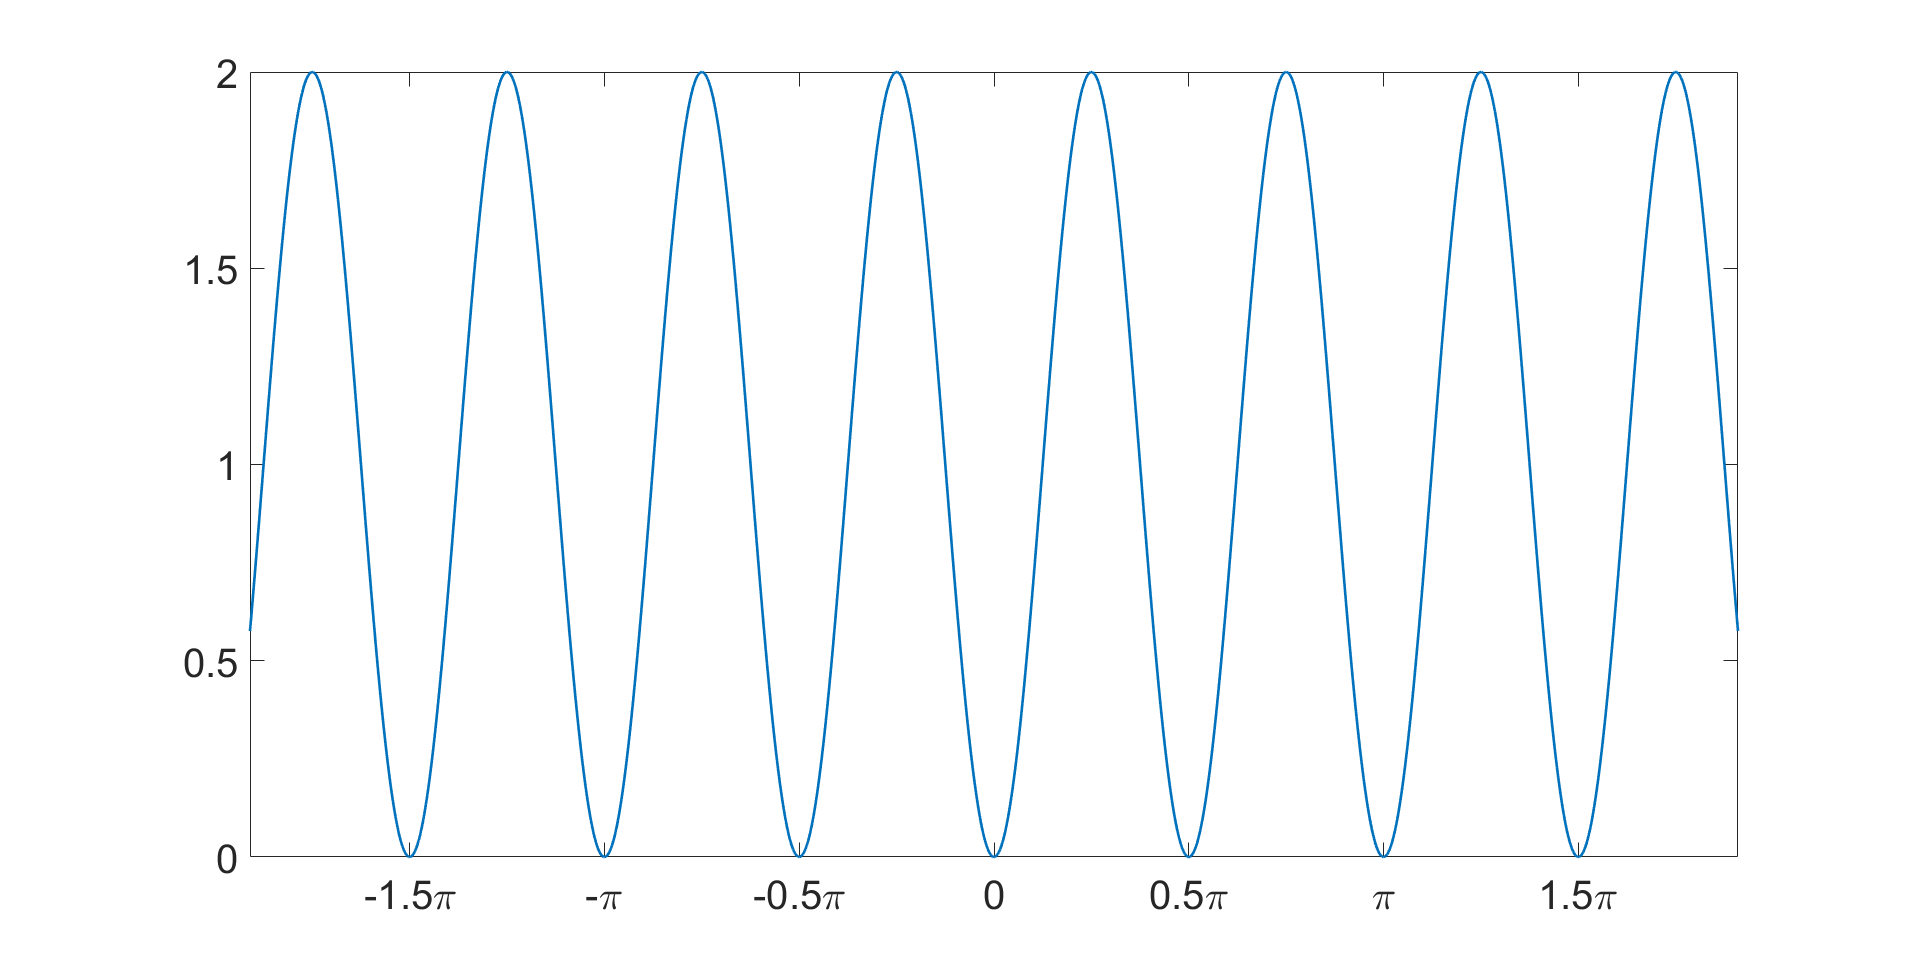
\includegraphics[width=12cm]{figures/seamless/angle_penalty_function.png}
\caption[The Angle Penalty Function]{A plot of the angle penalty function for a range of $\theta$ values. The penalty is zero for values of integer multiples of $\frac{\pi}{2}$, which represent a $\frac{\pi}{2}k$ rotation between the two half-edges, for $k \in \mathbb{N}$.}
\label{fig:angle_penalty}
\end{figure}
\paragraph{Length Penalty}
\label{paragraph:length_penalty_function_method}
We define the length penalty function $P_{length}$ as follows:
\begin{equation}\label{length_penalty}
\begin{split}
P_{\mathrm{length}}\left(e_i,e_j\right) = \left(\norm{e_i}_2^2 - \norm{e_j}_2^2\right)^2
\end{split}
\end{equation}
The length penalty measures the Euclidean length discrepancy between the two half-edges. It is a non-convex function (However, its Hessian is positive semi-definite almost everywhere) with multiple global minimum points associated with the function value of $0$. Therefore, It is easy to see that the length penalty is minimized when the length discrepancy between the two half-edges is absolutely zero, as required by the seamless condition. Figure \ref{fig:length_penalty} shows a plots of the length penalty function for a range of $\norm{e_i}_2^2$ and $\norm{e_j}_2^2$ values.
\begin{figure}[ht]
\centering
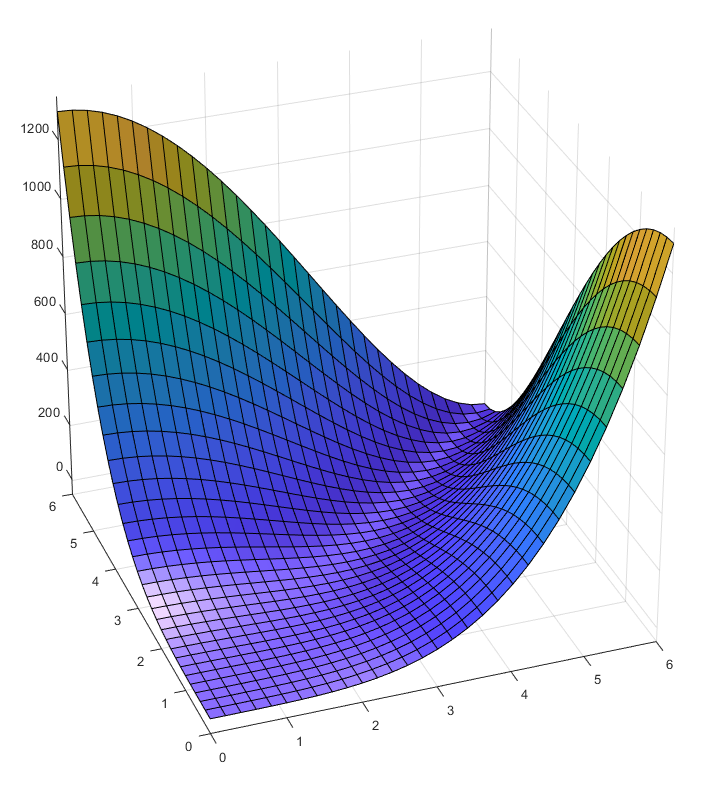
\includegraphics[width=8cm]{figures/seamless/length_penalty_function.png}
\caption[The Length Penalty Function]{A plot of the length penalty function. The penalty is zero along the $x=y$ line on the domain, where the lengths of the two half-edges are equal.}
\label{fig:length_penalty}
\end{figure}
% The length penalty measures the Euclidean length discrepancy between the two half-edges. It is a convex function (its Hessian is positive semi-definite) with multiple global minimum points associated with the function value of $0$. Therefore, It is easy to see that the length penalty is minimized when the length discrepancy between the two half-edges is absolutely zero, as required by the seamless condition.
\paragraph{Translation Penalty}
\label{paragraph:translation_penalty_function_method}
We define the translation penalty function $P_{\mathrm{translation}}$ as follows:
\begin{equation}\label{eq:translation_penalty}
\begin{split}
P_{\mathrm{translation}}\left(e_i,e_j\right) = \mathrm{sin} \Big( 2\pi\cdot\Delta_x\big(e_i,e_j\big) - \frac{\pi}{2}\Big) + \mathrm{sin} \Big( 2\pi\cdot\Delta_y\big(e_i,e_j\big) - \frac{\pi}{2}\Big) + 2
\end{split}
\end{equation}
Where $\Delta_x\big(e_i,e_j\big) = \mathrm{x}\left(v_i^1\right) - \mathrm{x}\left(v_j^1\right)$ and $\Delta_y\big(e_i,e_j\big) = \mathrm{y}\left(v_i^1\right) - \mathrm{y}\left(v_j^1\right)$ represent the Manhattan distance between the two twin-vertices $v^i_1$ and $v^j_1$, which is also, implicitly, the Manhattan distance between the two half-edges. Since the two sine terms in equation \ref{eq:translation_penalty} achieve their minimum value only for integer $\Delta_x$ and $\Delta_y$, it means that the function penalize non-integer Manhattan distances. Therefore, it is easy to see that the translation penalty is minimized when the two twin-vertices are integer distance apart, as required by the seamless condition. Figure \ref{fig:translation_penalty} shows a plot of the translation penalty function for a range of $\Delta_x$ and $\Delta_y$ values. Please note, equation \ref{eq:translation_penalty} yields only non-negative values due to the introduction of the $+2$ term.
\begin{figure}[ht]
\centering
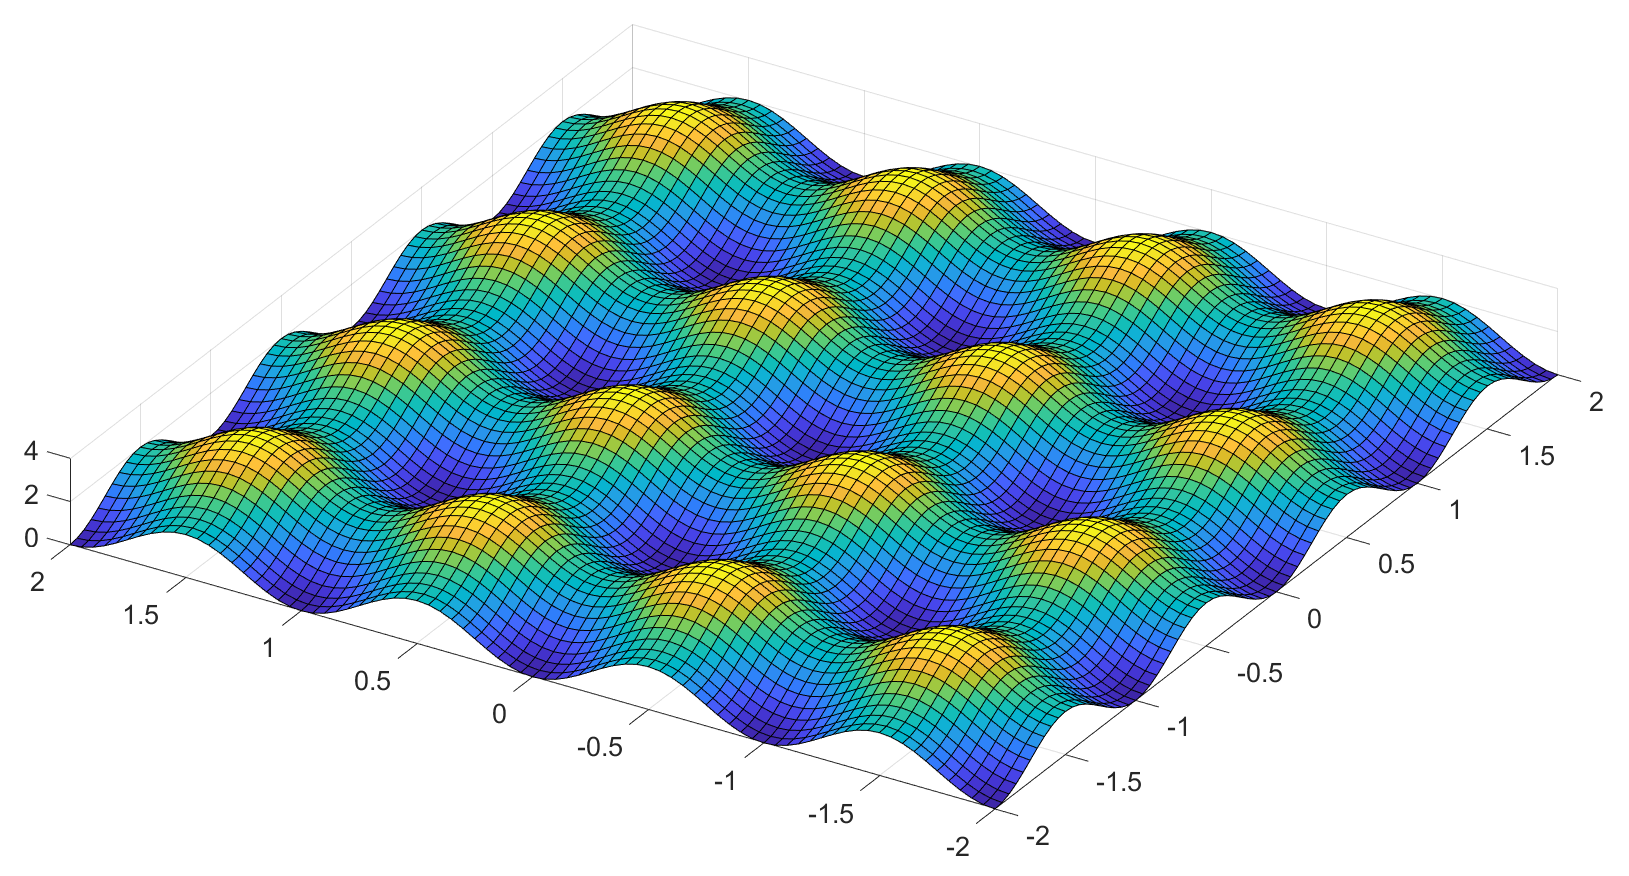
\includegraphics[width=13cm]{figures/seamless/translation_penalty_function.png}
\caption[The Translation Penalty Function]{A plot of the translation penalty function for a range of $\Delta_x$ and $\Delta_y$ values. As can be seen, global minimum points are located at integer locations, which represent integer translations.}
\label{fig:translation_penalty}
\end{figure}
\subsection{The Singular-Points Condition's Penalty Function}
\label{section:singular_points_penlaty_function_method}
The singular-points penalty function is applied on groups of twin-vertices on the parametrization domain, with non-zero angular defect (as defined in subsection \ref{section:singular_points_cond}). Given a group $S$ of twin-vertices that correspond to a singular point, the singular-points penalty function applied on that group is defined as follows:
\begin{equation}\label{eq:singular_points_penalty}
\begin{split}
P_{\mathrm{singular}}\left(S\right) = \sum_{u \in S} \bigg( \mathrm{sin} \Big( 2\pi\cdot\mathrm{x}\big(u\big) - \frac{\pi}{2}\Big) + \mathrm{sin} \Big( 2\pi\cdot\mathrm{y}\big(u\big) - \frac{\pi}{2}\Big) + 2 \bigg)
\end{split}
\end{equation}
Where $\mathrm{x}\big(u\big)$ and $\mathrm{y}\big(u\big)$ represent the domain coordinates of a twin-vertex in $S$. Since the two sine terms in equation \ref{eq:singular_points_penalty} achieve their minimum value only for integer $\mathrm{x}\big(u\big)$ and $\mathrm{y}\big(u\big)$, it means that it penalize non-integer locations of singular twin-vertices. Therefore, it is easy to see that the translation penalty is minimized when \textbf{all} twin-vertices in $V$ are located on integer locations, as required by the singular-points condition. Please note, equation \ref{eq:singular_points_penalty} yields only non-negative values due to the introduction of the $+1$ term for each sine term. Figure \ref{fig:singular_points_penalty_sine_term} shows a plot of a single sine term from the singular-points penalty function for a range of $\mathrm{x}$ (or $\mathrm{y}$) values. Figure \ref{fig:singular_points_penalty_minimum} illustrates an example where the penalty function converge to a local minimum, where all twin-vertices located at grid-point locations.
\begin{figure}[ht]
\centering
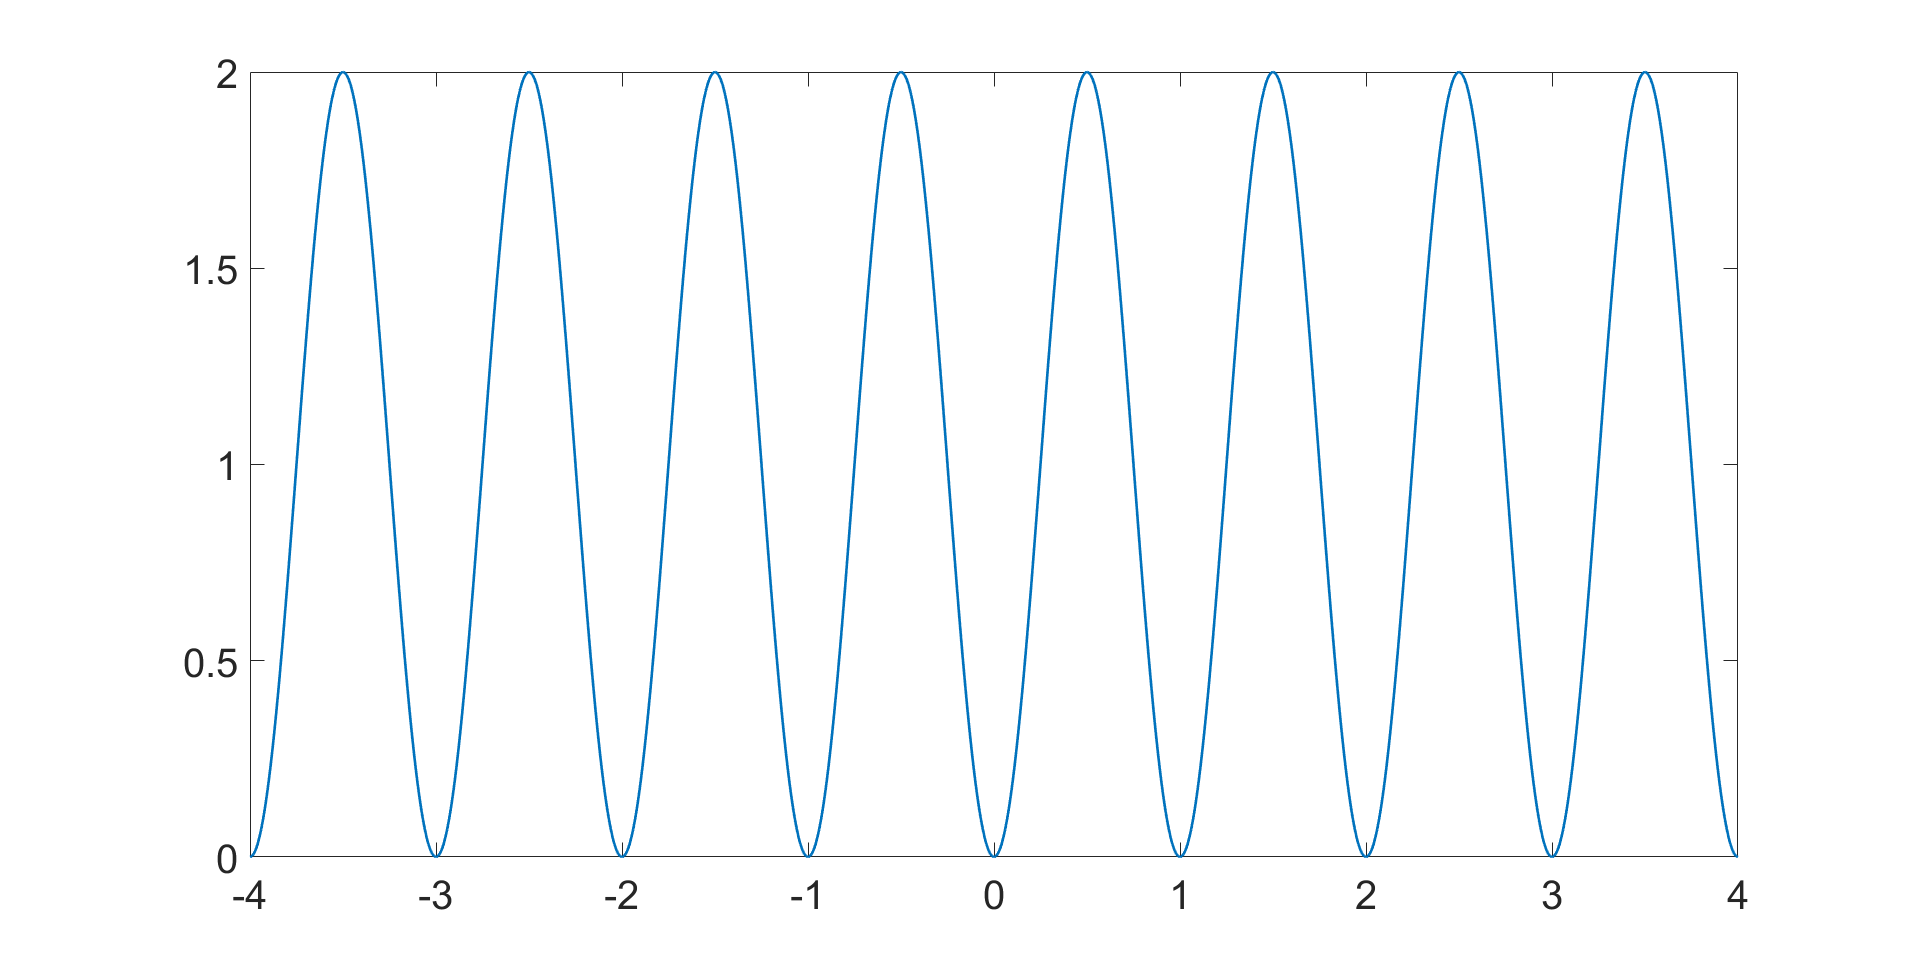
\includegraphics[width=13cm]{figures/singular_points/singular_points_penalty_function_sine_term.png}
\caption[The Singular-Points Penalty Function (Single Sine Term)]{A plot of a single sine term of the singular-points penalty function for a range of $\mathrm{x}$ (or $\mathrm{y}$). As can be seen, global minimum points are located at integer locations, which represent integer grid coordinates.}
\label{fig:singular_points_penalty_sine_term}
\end{figure}
\begin{figure}[ht]
\centering
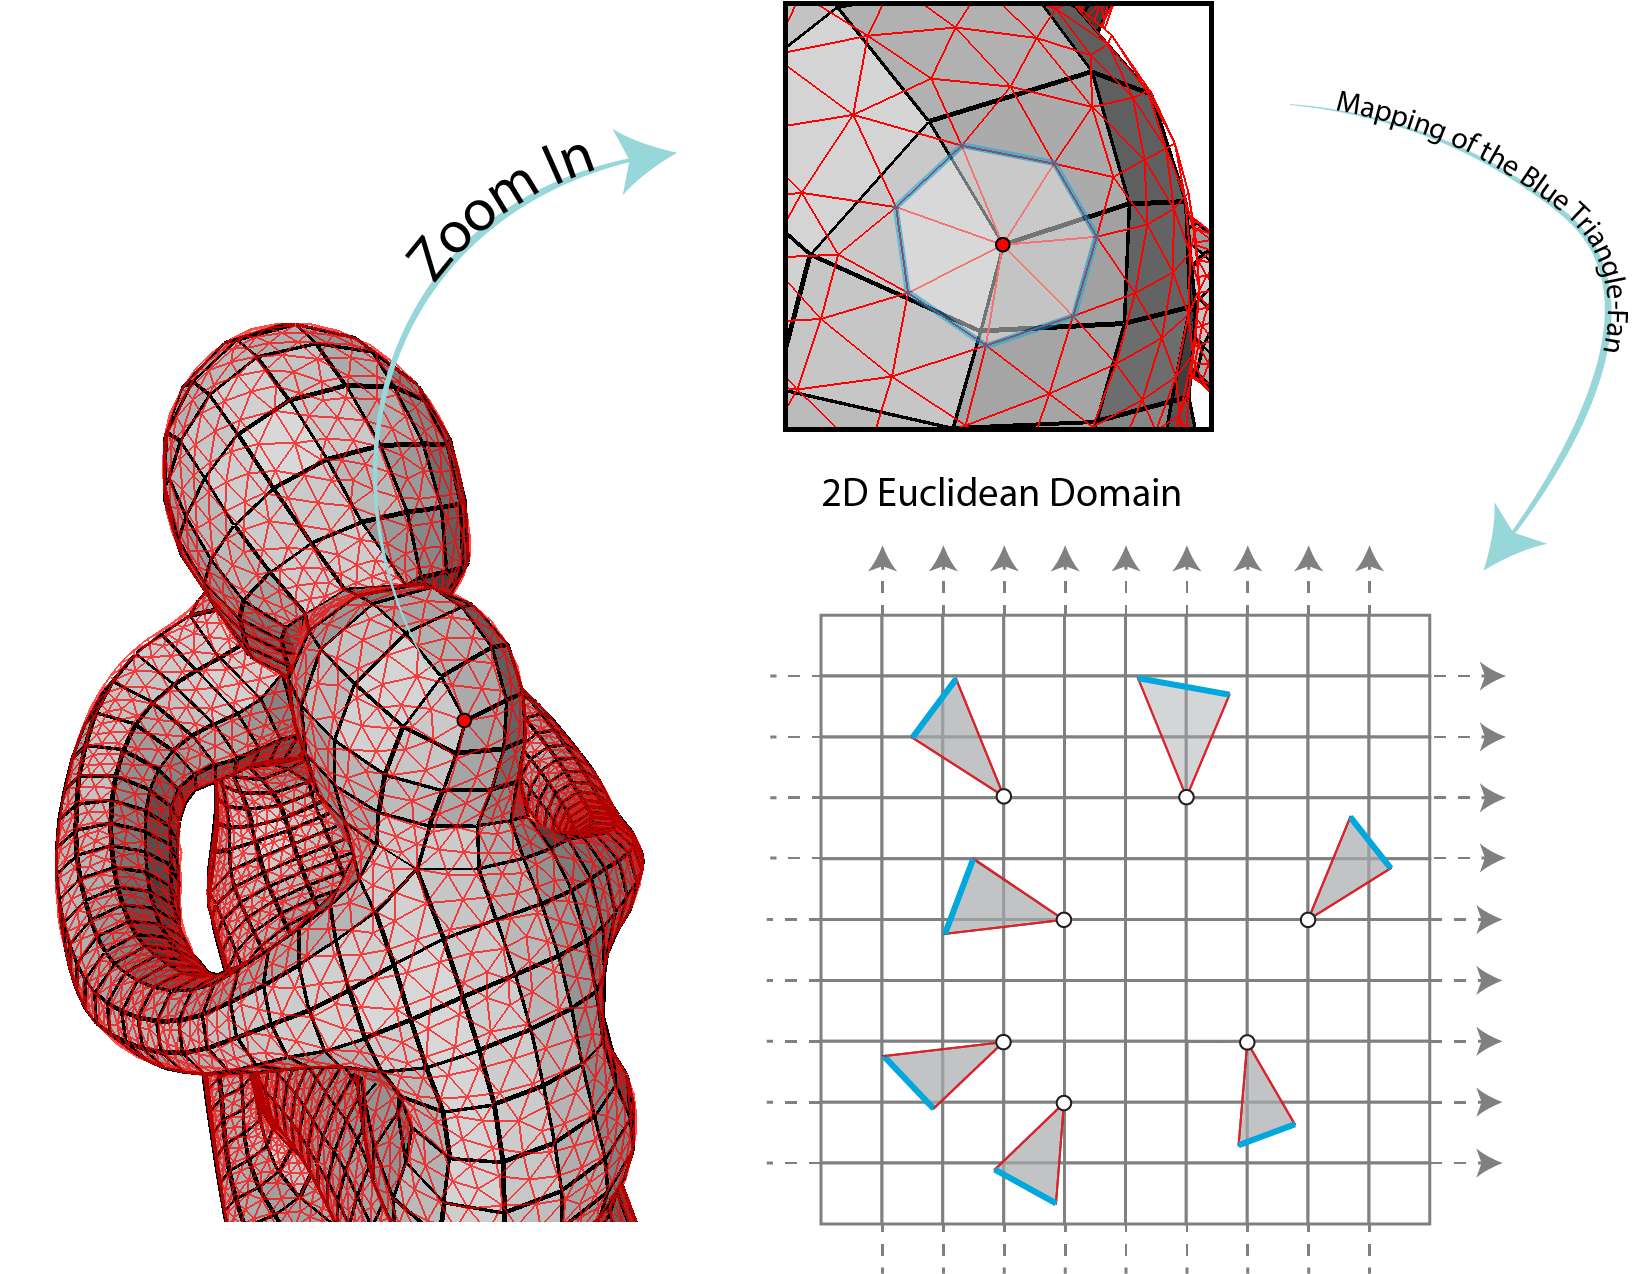
\includegraphics[width=12cm]{figures/singular_points/singular_points_penalty_function_minimum.png}
\caption[Singular-Points Penalty Function Global Minimum Example]{An example where the singular-points penalty function converges to a local minimum, when applied to a single singular-point. The red point on the mesh's surface represents a singular point of valence 3 (with respect to the black isolines), composed of a 7-facets blue triangle-fan. The corresponding triangle-soup on the parametrization domain satisfies the requirement that all twin-vertices of the singular-point are located on integer grid points. The sum of angles, adjacent to the group of twin-vertices, has a non-zero angular defect of $\frac{\pi}{2}$.}
\label{fig:singular_points_penalty_minimum}
\end{figure}
\subsection{The Consistent Orientation and Quad Distortion Conditions' Penalty Functions}
In this subsection, we denote by $J\left(f_i\right)$ the Jacobian of the linear part of the affine mapping of triangle $f_i$ on the parametrization domain. Inspired by \cite{Smith:2015} and \cite{Poranne:Autocuts:2017}, we express both the consistent-orientation condition and the requirement to minimize triangle distortion on the domain, by the following penalty function, which is known as the \emph{symmetric dirichlet energy}:
\begin{equation}\label{eq:orientation_and_distortion_penalty}
\begin{split}
P_{\mathrm{dirichlet}}\left(f_i\right) = P_{\mathrm{distortion}}\left(f_i\right) + P_{\mathrm{orientation}}\left(f_i\right)
\end{split}
\end{equation}
Where the left term is given by $P_{\mathrm{distortion}}\left(f_i\right) = \norm{J\left(f_i\right)}_F^2$ , the right term is given by $P_{\mathrm{orientation}}\left(f_i\right) = \norm{J\left(f_i\right)^{-1}}_F^2$, and $\norm{\cdot}_F^2$ is the squared Frobenius norm. It is known that for $A \in \mathbb{R}_{n \times n}$, the Frobenius norm of $A$ is a function of its singular values given by $\norm{A}_F^2 = \sqrt{\sum_{i=1}^{n} \sigma_i^2}$. Therefore, since $J\left(f_i\right) \in \mathbb{R}_{2 \times 2}$, we can rewrite $P_{\mathrm{dirichlet}}$ as follows:
\begin{equation}\label{eq:orientation_and_distortion_penalty_explicit}
\begin{split}
P_{\mathrm{dirichlet}}\left(f_i\right) = \sigma^2_1 + \sigma^2_2 + \sigma^{-2}_1 +\sigma^{-2}_2
\end{split}
\end{equation}
Where $\sigma_1$ and $\sigma_2$ are the two singular values of $J\left(f_i\right)$. Given that the mapping is initialized such that $\sigma_i > 0$, the dirichlet penalty function will prevent triangle flips since $\sigma^{-2}_i \xrightarrow[\sigma_i \to 0^+]{} \infty$, for $i \in \left\{1,2\right\}$. Moreover, the dirichlet penalty function is minimized when the Jacobian induce an isometric mapping, since its global minimum is achieved at $\sigma_1 = 1$ and $\sigma_2 = 1$. Figure \ref{fig:dirichlet_penalty_function} illustrate the dirichlet penalty function for a range of $\sigma_1$ and $\sigma_2$ values.
\begin{figure}[ht]
\centering
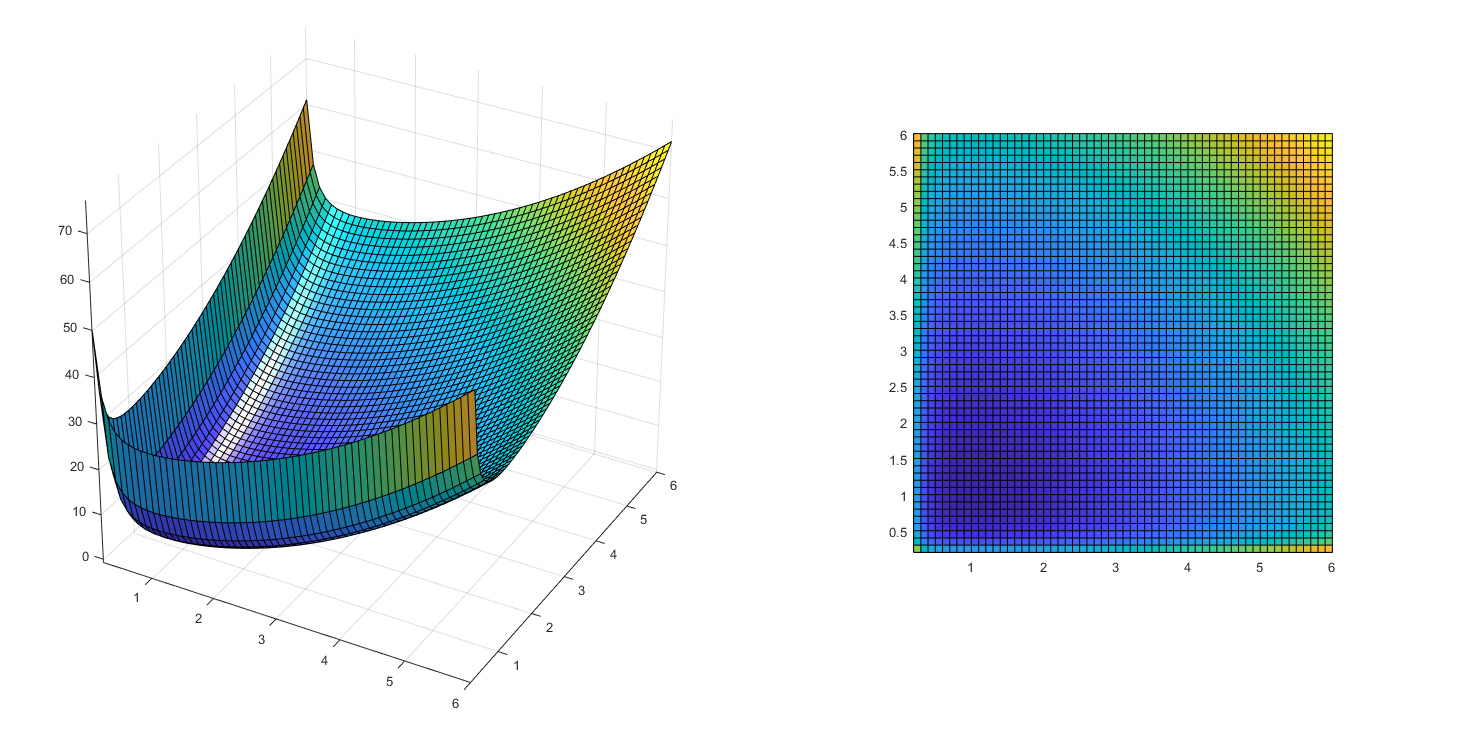
\includegraphics[width=16cm]{figures/dirichlet/symmetric_dirichlet_penalty_function.png}
\caption[The Symmetric Dirichlet Penalty Function]{On the left, a perspective view of the dirichlet penalty function is plotted. As can be seen, "walls" are formed along the positive $\sigma_1 = 0$ and $\sigma_2 = 0$ half-lines, infinitely penalizing an attempt to cross into an adjacent quadrant. On the right, a top view of the dirichlet penalty function is plotted, clearly showing that its global minimum is achieved at $\sigma_1 = 1$ and $\sigma_2 = 1$.}
\label{fig:dirichlet_penalty_function}
\end{figure}
\subsection{The Main Objective Function}
The main object function is a weighted sum of all penalty functions presented above, when applied to all target domain elements. It is given as follows:
\begin{equation}\label{eq:main_objective_function}
\begin{split}
P_{\mathrm{main}}\left(M_s\right) = &\underbrace{\sum_{e_i \sim e_j} \Big(w_{\mathrm{angle}} \cdot P_{\mathrm{angle}}\left(e_i,e_j\right) + w_{\mathrm{length}} \cdot P_{\mathrm{length}}\left(e_i,e_j\right) + w_{\mathrm{trans}} \cdot P_{\mathrm{trans}}\left(e_i,e_j\right)\Big)}_{\text{Weighted Seamless Condition}} + \\
&\underbrace{w_{\mathrm{singular}} \cdot \sum_{S_i} \Big(P_{\mathrm{singular}}\left(S_i\right)\Big)}_{\text{Weighted Singular Points Condition}} +
\\
&\underbrace{w_{\mathrm{dirichlet}} \cdot \sum_{f_i} \Big(A_{f_i} \cdot P_{\mathrm{dirichlet}}\left(f_i\right)\Big)}_{\text{Weighted Orientation and Distortion Condition}}
\end{split}
\end{equation}
Where $M_s = \left(V_s, E_s, F_s\right)$ is the domain triangle-soup of the input mesh (as explained in subsection \ref{sec:triangle_soup}), $e_i \sim e_j$ are two half-edges in $E_s$, $w_{\mathrm{angle}} \in \mathrm{R}$ is the angle penalty function weight, $w_{\mathrm{length}} \in \mathrm{R}$ is the length penalty function weight, $w_{\mathrm{trans}} \in \mathrm{R}$ is the translation penalty function weight, $S_i \subset V_s$ is a group of twin-vertices corresponding to a singular point, $w_{\mathrm{singular}} \in \mathrm{R}$ is the singular-points penalty function weight, $f_i \in F_s$ and $A_{f_i}$ are a triangle on the parametrization domain and its area , respectively, and $w_{\mathrm{dirichlet}} \in \mathrm{R}$ is the dirichlet penalty function weight. The tuple $\left(w_{\mathrm{angle}}, w_{\mathrm{length}}, w_{\mathrm{trans}}, w_{\mathrm{singular}}, w_{\mathrm{dirichlet}}\right)$ is controllable by the user and represents the core hyper-parameters of our system. The main objective function $P_{\mathrm{main}}$ is a non-convex multivariate scalar function, and our goal is to find a local minimum point that represents a configuration where the parametrization domain forms a valid quad-mesh when lifted onto the 3D input-mesh's surface.
\section{Optimization}
\label{section:optimization}
Since each individual penalty function is a smooth multivariate scalar function, we get that also $P_{\mathrm{main}}: \mathbb{R}^{2\abs{V_s}} \xrightarrow[]{} \mathbb{R}$ is a smooth multivariate scalar function. It has $2\abs{V_s}$ variables, since there are $\abs{V_s}$ vertices, and each vertex has two coordinates. Therefore, its gradient $\nabla P_{\mathrm{main}}: \mathbb{R}^{2\abs{V_s}} \xrightarrow[]{} \mathbb{R}^{2\abs{V_s}}$ is given by:
\begin{equation}\label{eq:main_objective_function_gradient}
\begin{split}
\nabla P_{\mathrm{main}}\left(M_s\right) = &\sum_{e_i \sim e_j} \Big(w_{\mathrm{angle}} \cdot \nabla P_{\mathrm{angle}}\left(e_i,e_j\right) + w_{\mathrm{length}} \cdot \nabla P_{\mathrm{length}}\left(e_i,e_j\right) + w_{\mathrm{trans}} \cdot \nabla P_{\mathrm{trans}}\left(e_i,e_j\right)\Big) + \\
&w_{\mathrm{singular}} \cdot \sum_{S_i} \Big(\nabla P_{\mathrm{singular}}\left(S_i\right)\Big) +
\\
&w_{\mathrm{dirichlet}} \cdot \sum_{f_i} \Big(A_{f_i} \cdot \nabla P_{\mathrm{dirichlet}}\left(f_i\right)\Big)
\end{split}
\end{equation}
By smoothness, we also get that the Hessian $\nabla^2 P_{\mathrm{main}}: \mathbb{R}^{2\abs{V_s}} \xrightarrow[]{} \mathbb{R}^{2\abs{V_s} \times 2\abs{V_s}}$ is given by:
\begin{equation}\label{eq:main_objective_function_gradient}
\begin{split}
\nabla^2 P_{\mathrm{main}}\left(M_s\right) = &\sum_{e_i \sim e_j} \Big(w_{\mathrm{angle}} \cdot \nabla^2 P_{\mathrm{angle}}\left(e_i,e_j\right) + w_{\mathrm{length}} \cdot \nabla^2 P_{\mathrm{length}}\left(e_i,e_j\right) + w_{\mathrm{trans}} \cdot \nabla^2 P_{\mathrm{trans}}\left(e_i,e_j\right)\Big) + \\
&w_{\mathrm{singular}} \cdot \sum_{S_i} \Big(\nabla^2 P_{\mathrm{singular}}\left(S_i\right)\Big) +
\\
&w_{\mathrm{dirichlet}} \cdot \sum_{f_i} \Big(A_{f_i} \cdot \nabla^2 P_{\mathrm{dirichlet}}\left(f_i\right)\Big)
\end{split}
\end{equation}
In other words, to calculate the gradient and Hessian of $P_{\mathrm{main}}$, it is enough to derive the gradient and Hessian of each individual penalty function, apply them to each domain element, and use the same weighted sum to calculate the end result. Full derivations of the gradient and Hessian of each penalty function is available in Appendix \ref{appendix:a}.

\noindent We find a local minimum of $P_{\mathrm{main}}$ by employing Newton's method with line-search. Given the parametrization domain's triangle-soup at the $i$th iteration $M_s^i = \left(V_s^i, E_s, F_s\right)$, we solve the linear system of equations $\nabla^2 P_{\mathrm{main}}\left(M_s^i\right) \cdot d^i = -\nabla P_{\mathrm{main}}\left(M_s^i\right)$ in order to find the current direction of descent $d^i$. Next, we perform a line-search, by iteratively searching for a scalar $\alpha^* > 0$ such that $P_{\mathrm{main}}\left(M_s^\alpha^*\right) < P_{\mathrm{main}}\left(M_s^i\right)$, where $M_s^\alpha^* = \left(V_s^i + \alpha^* d_i, E_s, F_s\right)$. When found, we update the locations of the triangle-soup's vertices (the explicit variables of our objective function) to $V_s^{i+1} = V_s^i + \alpha^* d_i$, to form a new triangle-soup state $M_s^{i+1} = \left(V_s^{i+1}, E_s, F_s\right)$. This process continues repetitively, until convergence (which is identified by $\norm{P_{\mathrm{main}}\left(M_s^i\right)}_2 < \epsilon_{\mathrm{mach}}$). The user can, at any moment in time, "play" with the problem's hyper-parameters, and steer the optimization process towards a better local minimum, according to his subjective requirements or technical/artistic opinion.

\noindent Since a 3D mesh is essentially a graph, it is characterized by sparse relationships between its nodes (vertices). Therefore, the Hessian $\nabla^2 P_{\mathrm{main}}$ is a sparse square matrix, which induce a sparse linear system of equations. We exploit this fact by using a parallel sparse linear solver (PARDISO \cite{SCHENK200169}) to quickly compute the direction of descent at each iteration.

\noindent Please note, in order for $d_i$ to be a descent direction, we have to make sure that $\nabla^2 P_{\mathrm{main}}\left(V_s^i\right)$ is positive semi-definite. Given the singular-value decomposition of an indefinite square matrix $A$ to be $A = USV^T$, its closest positive semi-definite matrix, in the Frobenius norm sense, is the matrix $\hat{A} = U\hat{S}V^T$ when $\hat{S}$ equal $S$ up to negative singular values, which are replaced with zeros. Therefore, since $\nabla^2 P_{\mathrm{main}}\left(V_s^i\right)$ is most likely to be an indefinite matrix, since we're solving a non-convex problem, we would like to find its closest positive semi-definite matrix, as use it as a replacement for the original Hessian. However, since the time complexity of singular-value decomposition is cubic, it become quite costly even for small meshes of a few hundreds vertices. Therefore, a more efficient approach would be to replace the Hessian of each individual penalty function with its closest positive semi-definite version. That way, we would have to compute singular-value decompositions of fixed sized matrices (the seamless condition's penalty functions accept a vector of size 8 as input, and therefore their Hessian is of size $8 \times 8$). Since the sum of positive semi-definite matrices yields a positive semi-definite matrix, we are guaranteed to get a positive semi-definite when summing-up the tweaked Hessians of all individual penalty functions.
\section{Initialization}
\label{section:initialization}
We cut the input triangle-mesh open by isometrically mapping its dual spanning tree to the parameterization plane as a triangle-soup. We first map an arbitrary initial triangle to the parameterization plane. Next, we map to the plane all adjacent triangles of the initial triangle, such that adjacent triangles on the mesh surface share an edge on the 2D domain. We continue this process for the next layer of neighbours, till we map the whole input mesh. Figure \ref{fig:initialization} visualize the initialization process.
\begin{figure}[ht]
\centering
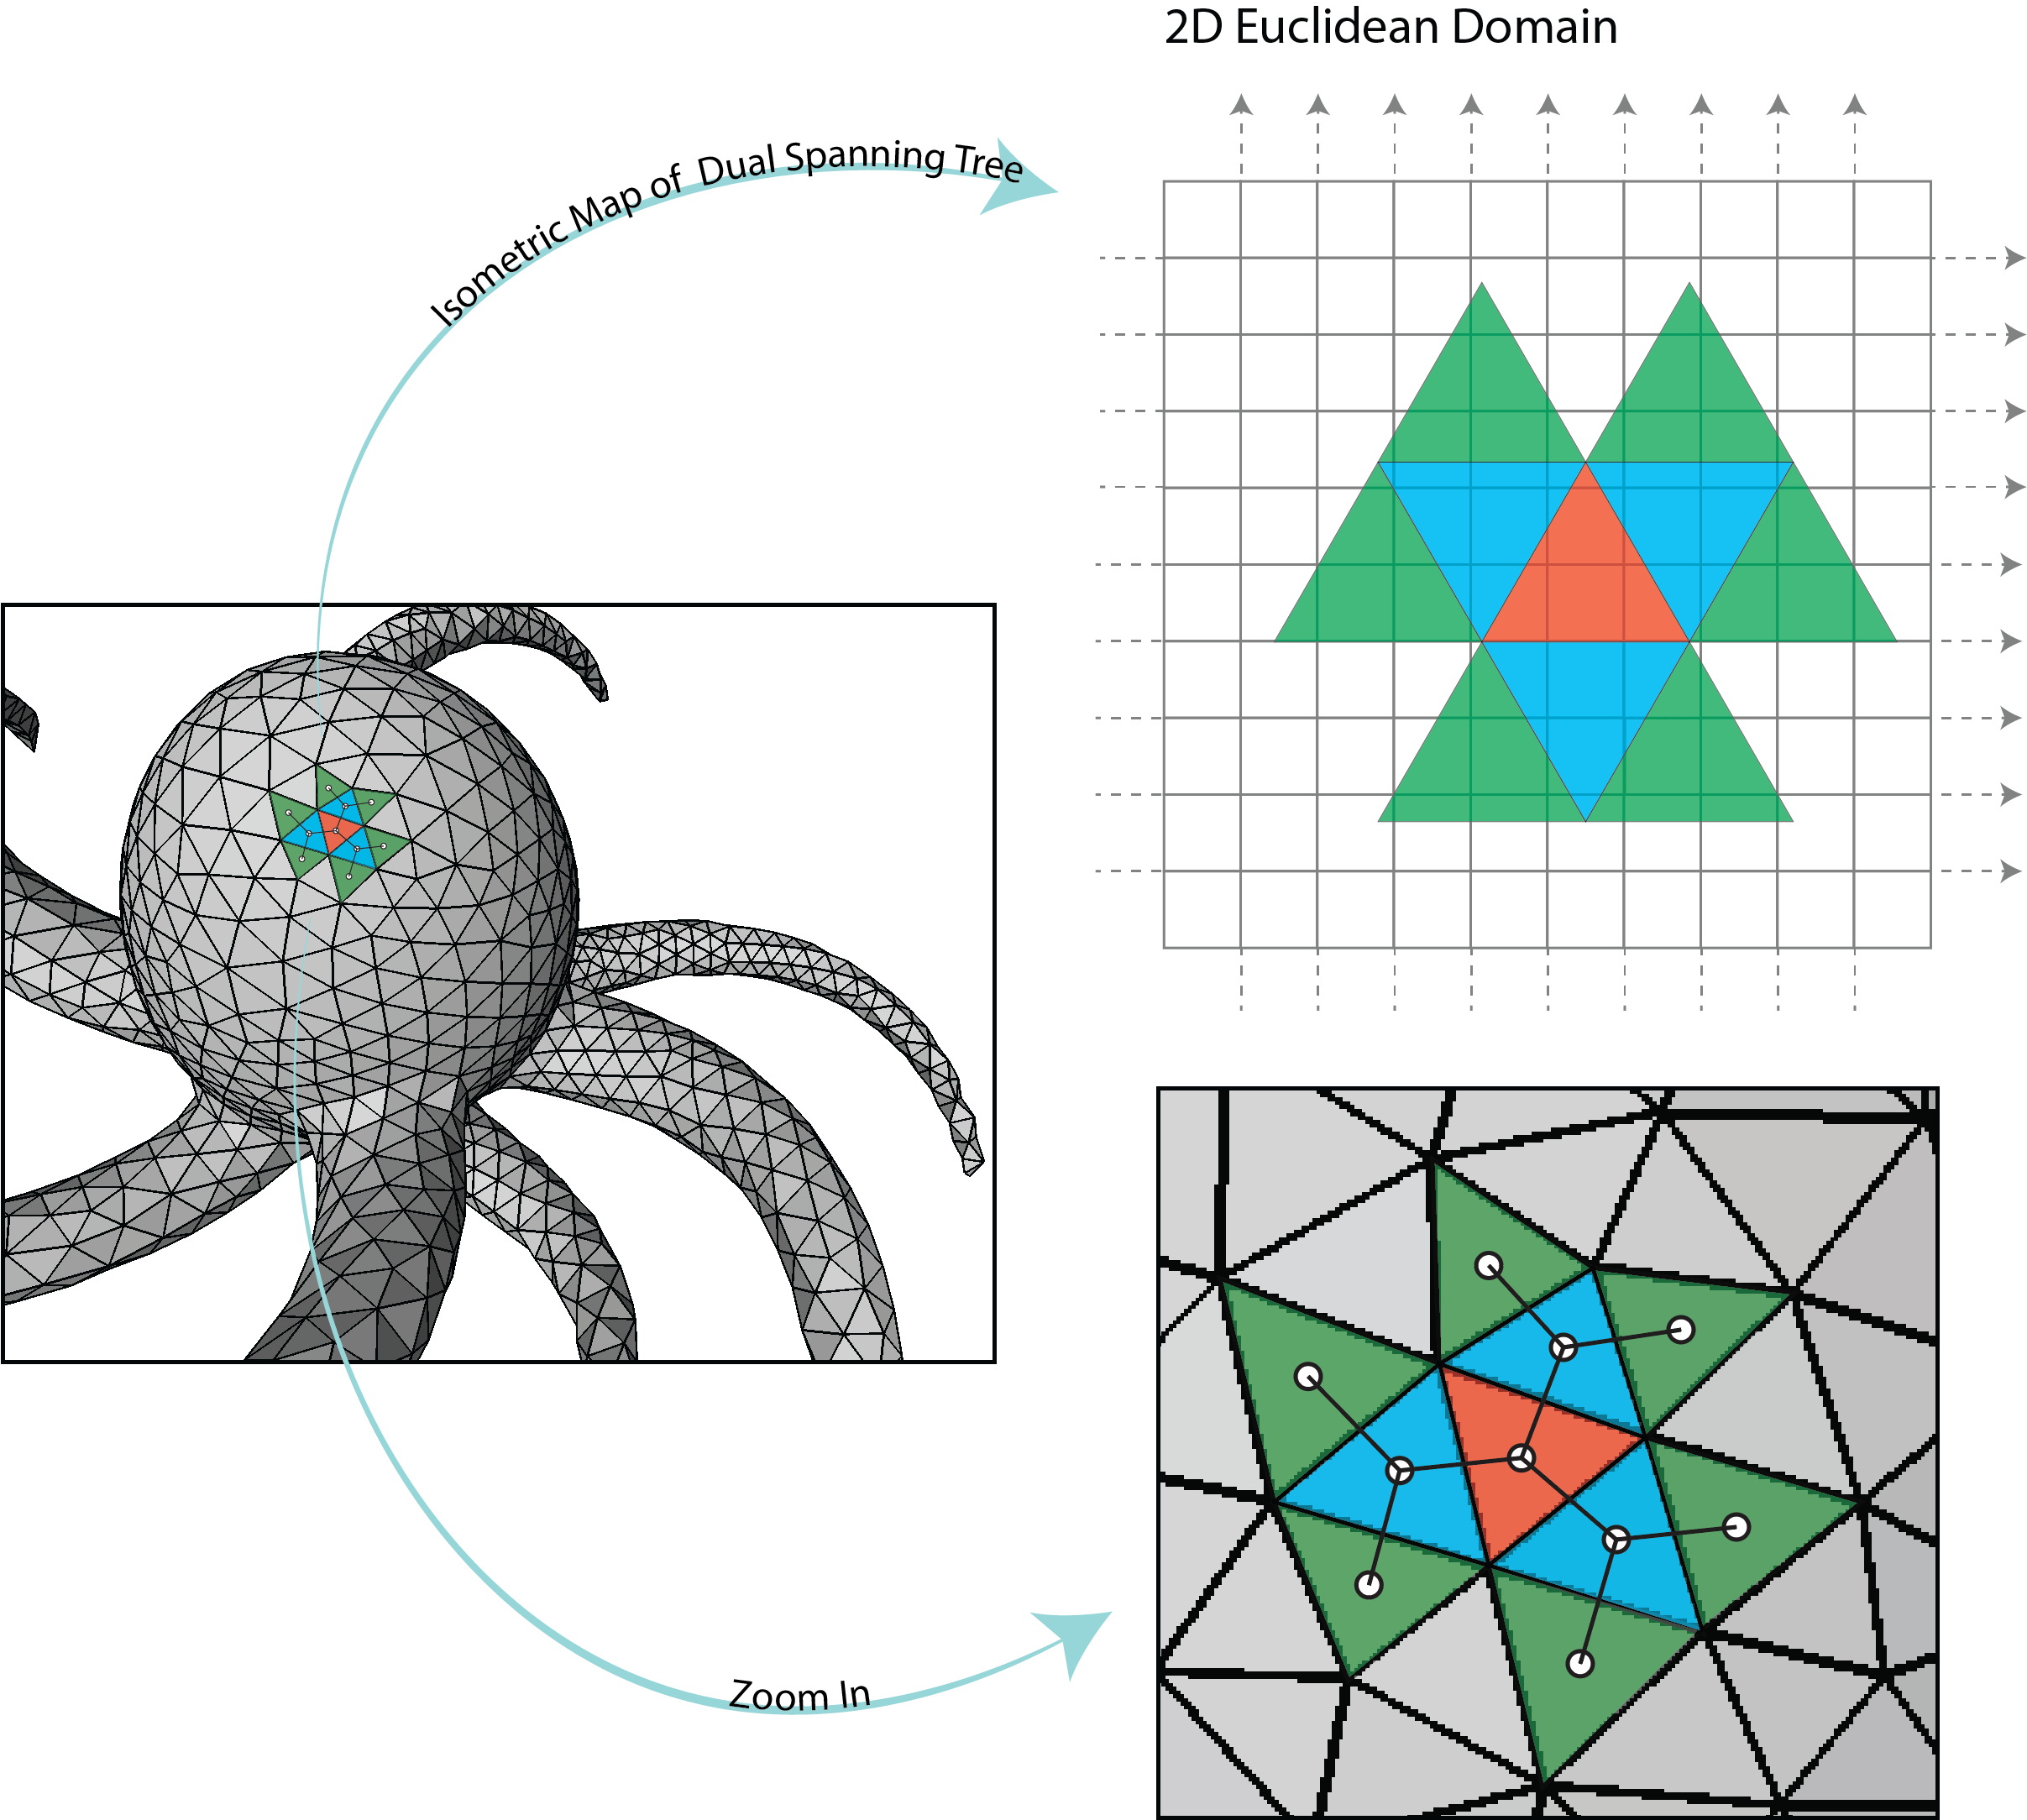
\includegraphics[width=13cm]{figures/initialization.png}
\caption[Triangle Soup Initialization]{An example of isometric map of the dual tree. The red triangle is chosen arbitrarily as the spanning tree root, and is isometrically mapped from the mesh onto the parametrization domain. Next, its immediate neighbours, the blue triangles, are copied isometrically onto the domain, such that adjacent edges on the mesh are adjacent also on the domain. The green triangles are the next layer of triangles to be copied, and so on until all mesh triangles are mapped.}
\label{fig:initialization}
\end{figure}
\section{Graphic User Interface}
\label{section:graphic_user_interface}
We designed a proof-of-concept interactive tool which accepts an input triangle-mesh, and smoothly transform it into a quad-mesh by minimizing the main objective function, guided by the user's interaction with the system's hyper-parameters. The user-interface front-end is based on web-technologies, and thus can be easily extended and adapted to new scenarios and requirements. The tool's back-end is written in modern C++ and is using Intel's MKL PARDISO (PARallel DIrect SOlver) to factorize the main objective's Hessian matrix, and solve the sparse linear system of equations, taking advantage of a multicore CPU environment. A short introduction video is available in  \href{https://youtu.be/1zP5KO8EwHQ}{this} link, and the project's GitHub repository is available \href{https://github.com/HaifaGraphics/RDS/tree/royv}{here}. Figure \ref{fig:gui} gives a short explanation of the main components of the graphic user interface.
\begin{figure}[ht]
\centering
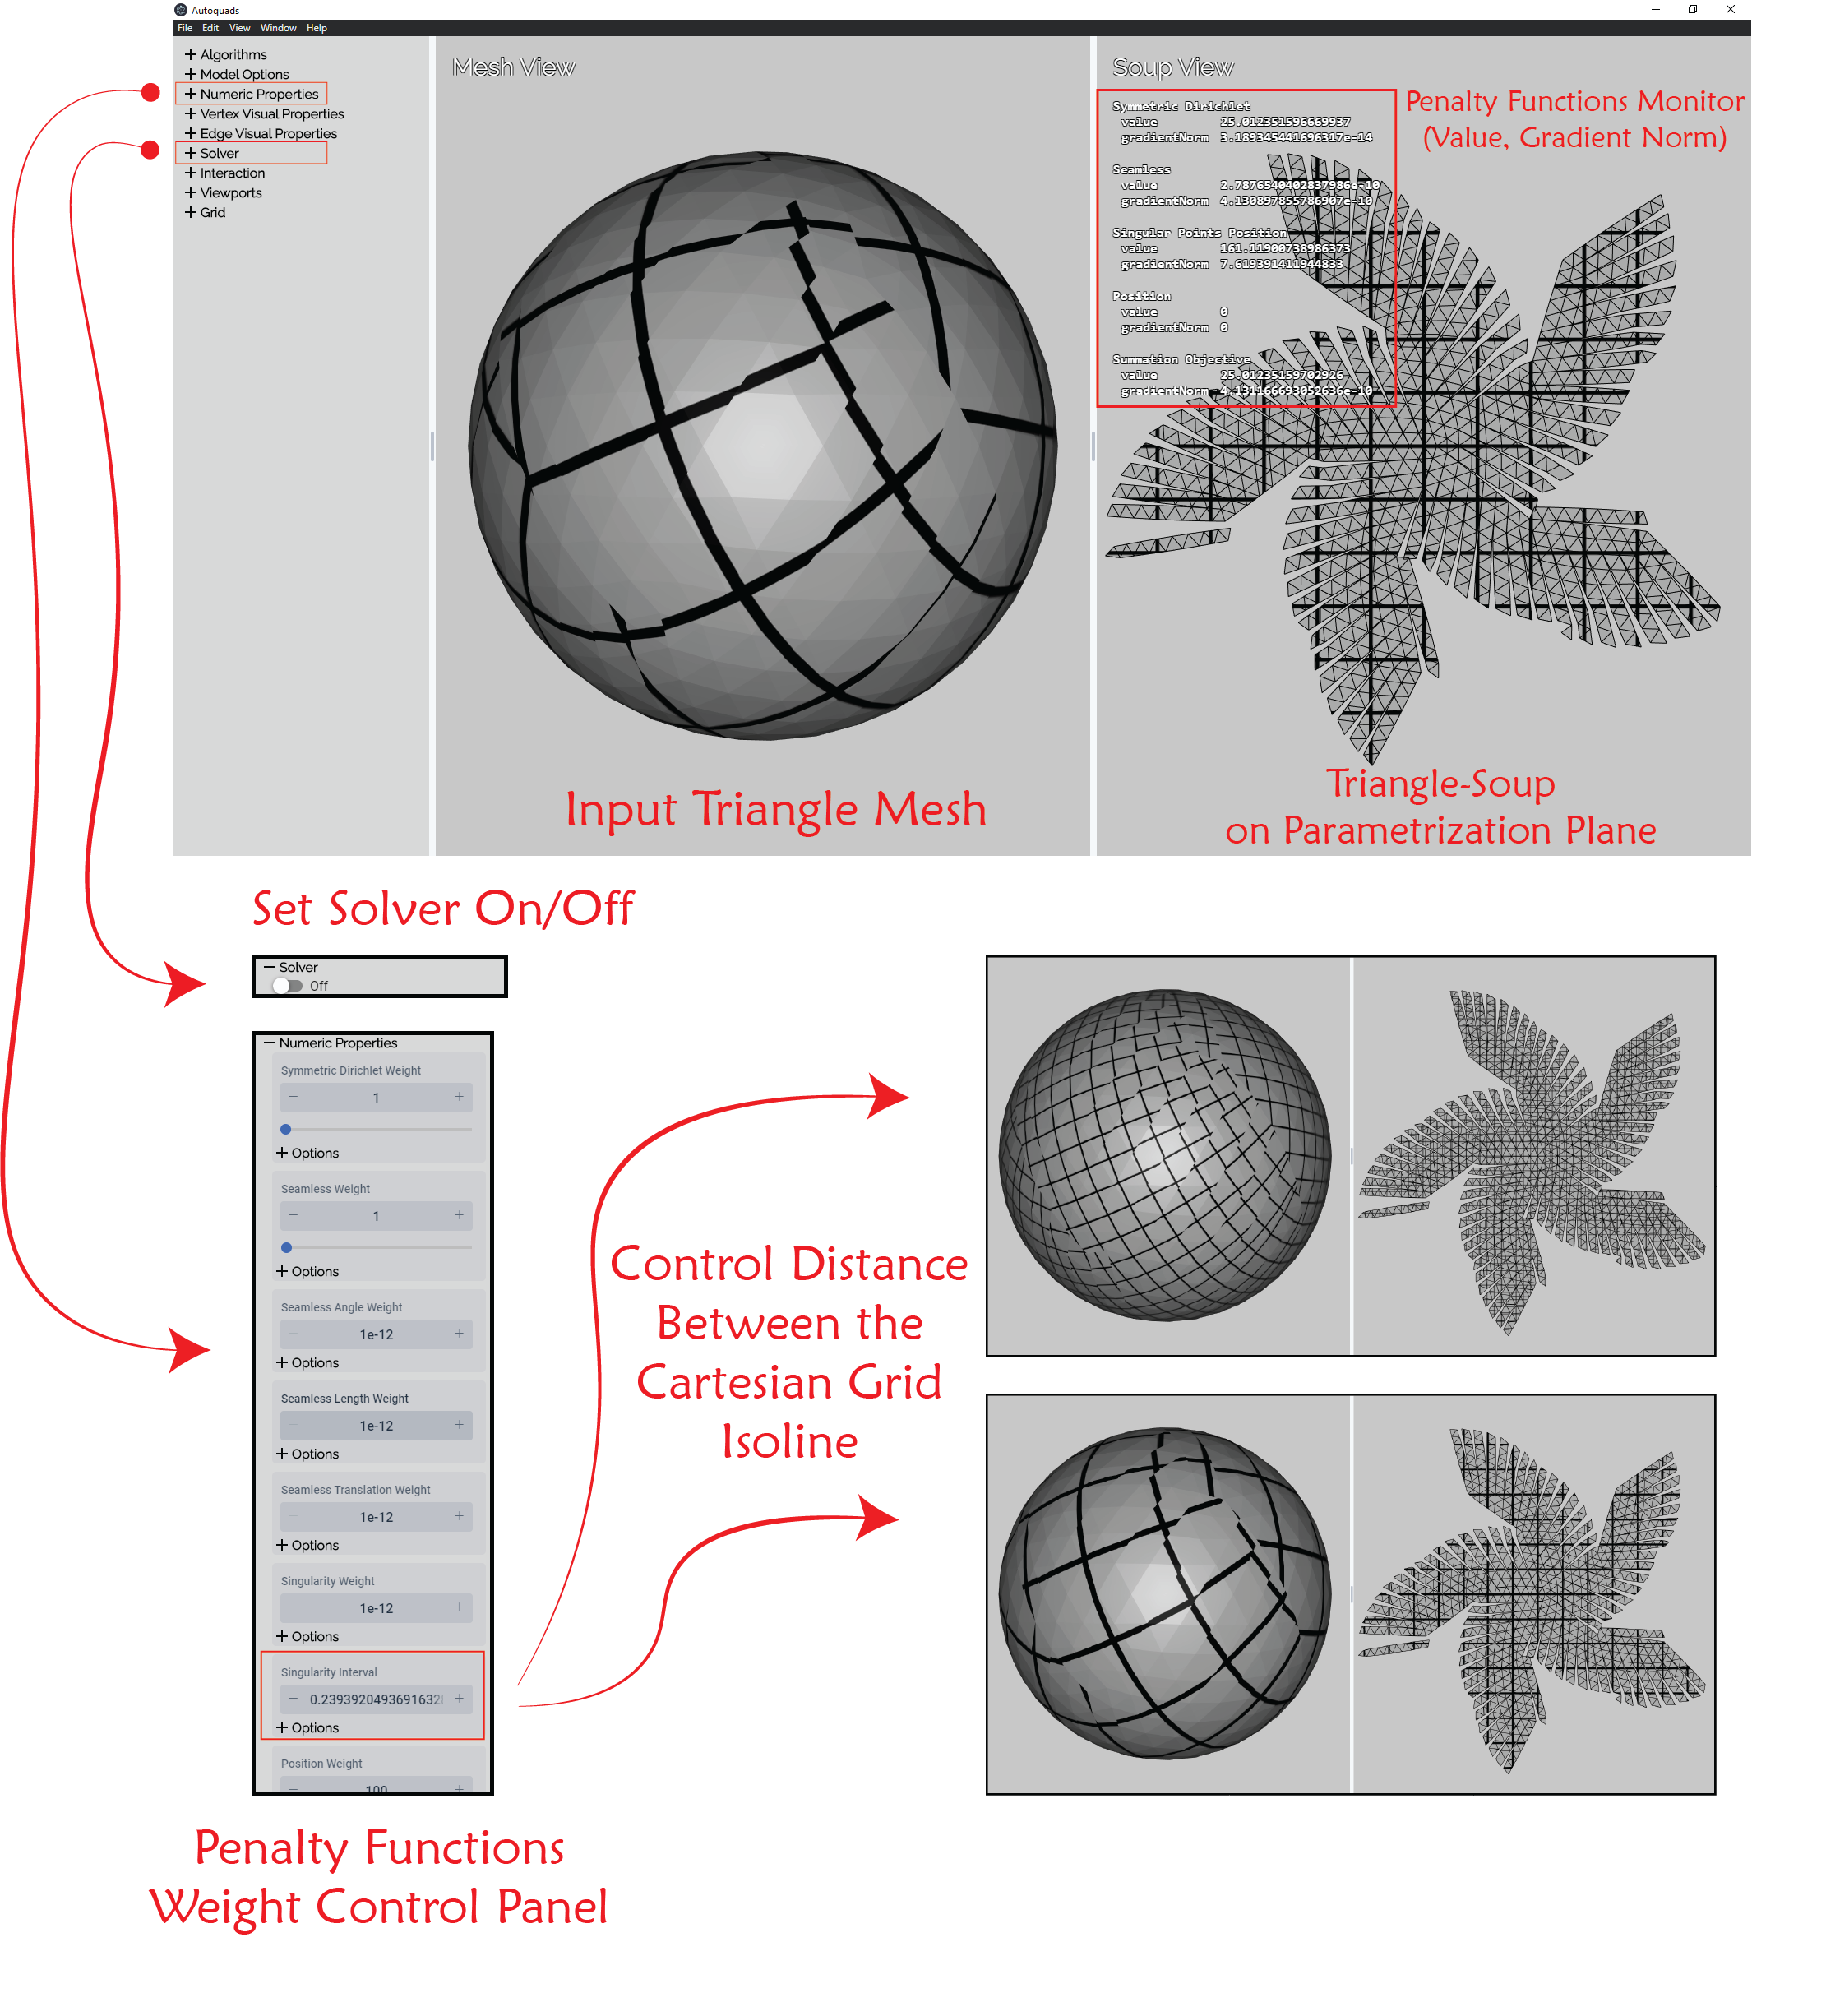
\includegraphics[width=15cm]{figures/gui.png}
\caption[Graphic User Interface]{The basic elements of graphic user interface. [TOP] A split screen is displayed to the user, where its left pane renders the 3D surface of the input triangle-mesh, and the right pane renders the triangle-soup on the parametrization domain. The parametrization domain is tessellated with the Cartesian grid's isolines. The portion of the Cartesian grid covered by soup triangles is used as a texture that is mapped back onto the 3D mesh surface to form a quad-mesh. A monitor is transparently overlayed on top of the right pane to reflect the current state of each penalty function.  [BOTTOM] The user can pause/resume the optimization process, and control the weights of the penalty functions. The user can also control the spacing between the Cartesian grid's isolines, and thus control the quads size.}
\label{fig:gui}
\end{figure}